\section{Molecules and their representations}
\label{sec:background:mols}

The question ``what is a molecule'' is surprisingly nuanced and hard to answer
(see \S\ref{sec:what are molecules}).
All algorithms in this thesis interact with molecules only via some \emph{representation},
and therefore we denote by $\molspace$ the space of molecule representations.
Since the distinction between molecules and their representations
is not critical in this thesis, $\molspace$ will equivalently be referred to as simply
the space of molecules.\footnote{
    A more rigorous definition is as follows:
    let $\mathfrak{M}$ denote some abstract space of molecules,
    and let $r:\mathfrak M\mapsto \mathcal X$ map molecules to some representation
    space $\mathcal X$ with an equivalence relation.
    Define an equivalence relation $\sim$ between molecules by $m_1\sim m_2$ if
    $r(m_1)=r(m_2)$.
    $\molspace$ is then the quotient space $\mathfrak M / \sim$.
}

The fundamental representation used in this thesis is
\emph{standardized graphs}:
a set of nodes representing atoms and a set edges representing bonds between them.
Nodes possess a small set of discrete labels including atom type, electric charge,
and stereochemistry tags.\footnote{
    \citet[page~960]{zumdahl2006chemistry}
    defines \emph{stereoisomerism} as
    \begin{quote}
        where all the bonds in the isomers are the same but the spatial arrangements of the atoms are different.
    \end{quote}
    The general term ``stereochemistry tags'' is used in this thesis to refer to information
    used to disambiguate between stereoisomers.
    The exact specification of these tags is not important to the key ideas of this thesis,
    we simply emphasize that they exist.
}
Edges possess labels indicating bond types.
Examples of molecules are shown in Figure~\ref{fig:background-example-molecules}.
The \emph{standardization} refers to the resolution of a small number of equivalences between molecular graphs,
chiefly multiple ways of denoting bonds in aromatic rings.
The precise details of this standardization are not important to the key ideas of this thesis;
in practice it is delegated to third-party python packages.

\begin{figure}
    \centering
    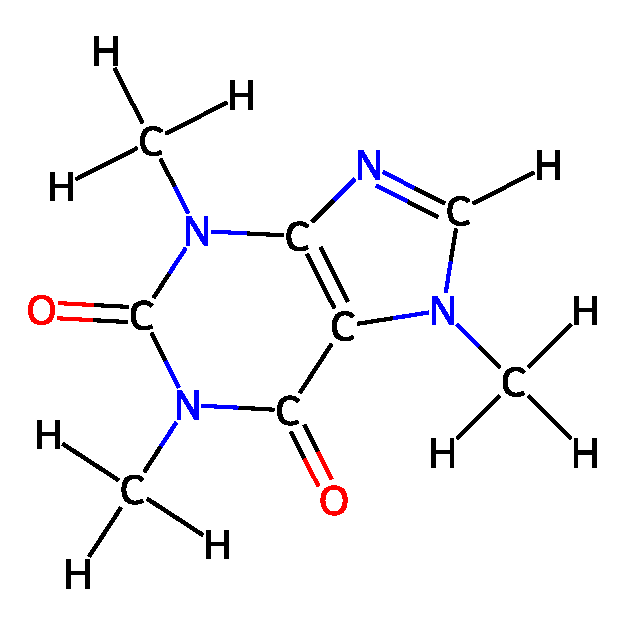
\includegraphics[width=0.4\textwidth]{caffeine-withHs.pdf}
    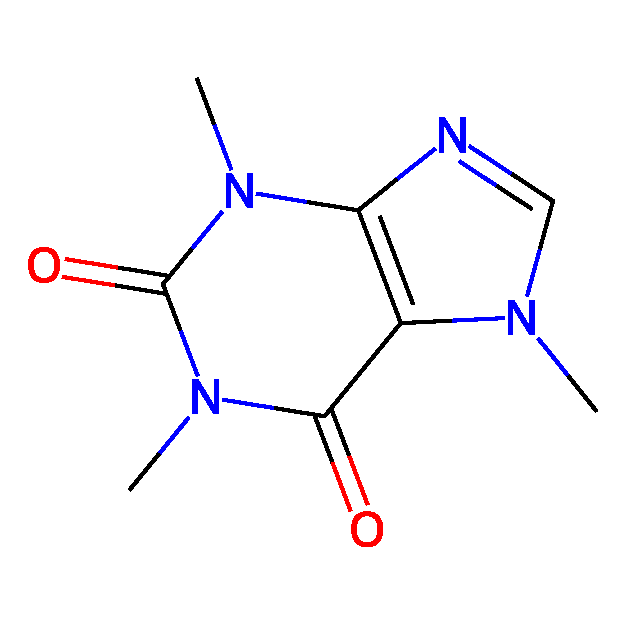
\includegraphics[width=0.4\textwidth]{caffeine-noHs.pdf}
    \caption[Graph of caffeine molecule.]{
        Left: graph for the molecule caffeine.
        Right: the \emph{skeletal formula} of the same graph:
        a simplified representation of the molecule which omits hydrogen atoms
        (whose presence can be inferred from the valency of the other atoms)
        and implicitly includes carbon atoms at the end of lines.
        Non-carbon atoms are labelled explicitly.
        This representation will be used in the remainder of the thesis.
    }
    \label{fig:background-example-molecules}
\end{figure}

With the exception of stereochemistry labels,
note that this representation excludes 3D descriptors of molecular structure,
despite molecules fundamentally being 3D objects.
This choice is made because in many practical applications one lacks both knowledge and control of a molecule's 3D structure
(the structure is determined by physics and the nanoscopic size of molecules preclude directly observing it).
Even when 3D structures can be inferred, the inability to freely \emph{control}
a molecule's 3D structure means this information is better viewed as a value calculated from the representation
rather than a fundamental property of the representation itself.

Note that for some problems,
only a subset of $\molspace$ is of interest.
In this case, we define $\amolspace\subseteq\molspace$ to be the set of \emph{accessible}
molecules for a given problem.
The exact nature of $\amolspace$ will be unique to each problem,
but could for example represent molecules which are purchasable
or molecules synthesizable within a fixed number of steps.
Many algorithms presented in this thesis are agnostic to the exact definition
of $\amolspace$ and it will therefore not be defined beyond simply being a subset of $\molspace$.
More specific definitions $\amolspace$ will be given when appropriate,
but should be understood to apply only within that specific section or chapter.

Although standardized graphs can sometimes be used directly as inputs to algorithms
(e.g.\@ in the form of a node list and an adjacency matrix),
it is often useful to post-process
these graphs into secondary, downstream representations
which are either not graph-structured or which yield additional information.
The remainder of this section will therefore introduce
common representations derived from graphs.
A more comprehensive introduction can be found in numerous review articles
\citep{david2020molecular,wigh2022representation,mcgibbon2023smol-representation}.

\subsection{Vector-valued \emph{descriptors}}

A molecular ``descriptor'' typically refers to some kind of real or integer quantity which can be computed from a graph.
Examples of simple descriptors are the number of atoms in a molecule,
the number of rotatable bonds, or the number of rings.
As of the writing of this thesis, the popular python package \texttt{rdkit}
provides over 200 structural descriptors of varying complexity.\footnote{
    See Greg Landrum's \href{https://greglandrum.github.io/rdkit-blog/posts/2022-12-23-descriptor-tutorial.html}{blog post from 2022-12-23}
    for details.
}
These descriptors can be selected and concatenated to form a fixed-length
vector representation of a molecule. 
Such representations were arguably more popular when machine learning was dominated by hand-engineered features,
and more broadly can be used when chemists' domain knowledge is sufficient to extract meaningful features for a given task.
However, this is not usually the case, and therefore such descriptors tend to be used only for naive baselines
and for heuristics such as ``Lipinski's rule of five'' \citep{lipinski2001experimental}.

\subsection{Vector-valued \emph{embeddings}}

Another approach to represent molecules as fixed-length vectors is to use the output of
machine learning models, most commonly neural networks.
We call such representations \emph{embeddings}.
Deferring the introduction of potential embedding models to \S\ref{sec:background:deep learning for molecules},
embeddings can be abstractly viewed as the output of functions $f_{\bm{\theta}}:\molspace\mapsto\R^m$
with parameters $\bm{\theta}$.
In principle there is no difference between embeddings and the ``descriptors''
introduced previously (both are vectors in $\R^m$).
However, in practice embeddings require model selection,
and unlike descriptor vectors individual dimensions of embeddings do not have a straightforward interpretation.
For this reason subsequent chapters will distinguish ``embedding'' vectors from ``descriptor'' vectors.

\subsection{String representations}
\label{sec:background:string-reps}

Any representation of molecules as sequence of discrete ``tokens'' (e.g.\@ letters of the alphabet)
can be considered a \emph{string representation}.
At present, the most popular and well-established string representation is unquestionably SMILES.
At a high level, a SMILES representation of a molecule marks a continuous ``path'' through a molecule
along bonded atoms, using parentheses `()' to denote branches from the path and numbers
to mark ring closures.
A simple example of a SMILES string is shown in Figure~\ref{fig:smiles-example}.
Because converting molecular graphs to/from SMILES representations
is handled by third-party python packages,
the precise details of SMILES syntax is not important in the context of this thesis
(although it is explained in more detail by \citet{weininger1988smiles}).
Only a few properties are important to understand subsequent material in this thesis:
\begin{enumerate}
    \item SMILES strings are formed from a fixed set of tokens,
        but not all arrangements of these tokens form a valid SMILES string.
        This sometimes necessitates ``validity checks''.
    \item Molecules can have multiple associated SMILES strings,
        which are formed by traversing a molecule's atoms in a different order.
        However, each SMILES string corresponds to only one graph.
        Therefore, the relationship between SMILES and graphs is a ``many to one'' mapping.
    \item It is possible to define \emph{canonical} SMILES such that there is a one-to-one relationship between molecular graphs and canonical SMILES.
        Algorithms to canonicalize SMILES are included in third-party libraries.
        This allows for collections of molecules to be stored as a set of canonical SMILES.
\end{enumerate}

\begin{figure}
    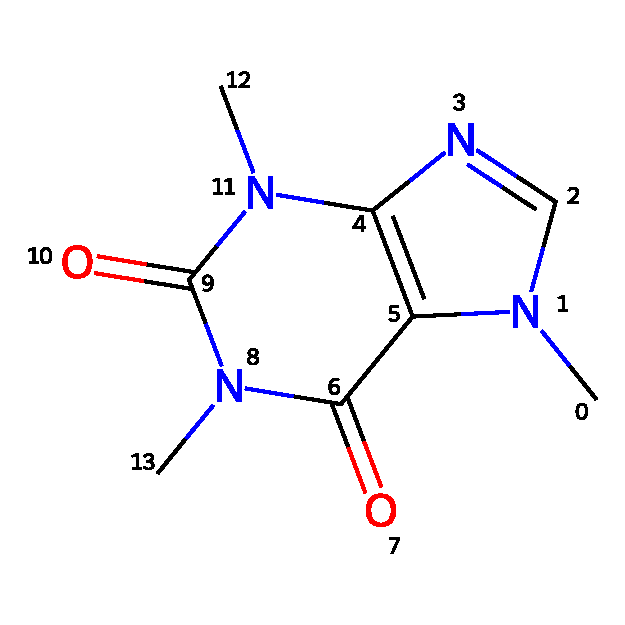
\includegraphics[width=0.4\textwidth]{caffeine-atom-indices.pdf}
    \begin{minipage}[b][0.4\textwidth][c]{0.55\textwidth}
        \begin{center}
            \begin{equation*}
                \setlength\arraycolsep{0pt}
                \begin{array}{cccccccccccccccccccccccccccc}
                        \texttt{C} & \texttt{N} & \texttt{1} & \texttt{C} & \texttt{=} & \texttt{N} & \texttt{C} & \texttt{2} & \texttt{=} & \texttt{C} & \texttt{1} & \texttt{C} & \texttt{(} & \texttt{=} & \texttt{O} & \texttt{)} & \texttt{N} & \texttt{(} & \texttt{C} & \texttt{(} & \texttt{=} & \texttt{O} & \texttt{)} & \texttt{N} & \texttt{2} & \texttt{C} & \texttt{)} & \texttt{C} \\
                        0          &      1     &            &          2 &            &          3 &     4      &            &            & 5          &            & 6          &            &            & 7          &            & 8          &            &       9    &            &            &     10     &            & 11         &            &  12        &            & 13
                    \end{array}
            \end{equation*}
        \end{center}
    \end{minipage}
    \caption[Explanation of SMILES string for caffeine]{
        Explanation of SMILES string for caffeine.
        The graph structure of caffeine is shown on the left, with all (non-hydrogen) atoms given an index.
        The SMILES string for caffeine is shown on the right.
        The numbers beneath each character indicate the corresponding atom index.
        Roughly, the string is formed by starting at atom $0$, traversing the right-hand ring to atom 5,
        then traversing the left hand ring to atom 12, and finally to the branching atom 13.
    }
    \label{fig:smiles-example}
\end{figure}

Other string representations exist to handle shortcomings of SMILES strings.
International Chemical Identifier (InChI) strings are more standardized
and use a hierarchical encoding to embed optional metadata such as stereochemistry tags,
but are not easy for humans to parse \citep{heller2015inchi}.
SELFIES are designed so that every arrangement of tokens from their alphabet forms a valid molecule
\citep{krenn2020self,krenn2022selfies}.
However, neither of these additional properties are useful for the works presented in this thesis,
thus these alternative representations are not used.

More generally, one may wonder why one would bother representing molecules as strings instead of graphs
given that such representations not only add no new information beyond the connectivity,
but arguably \emph{obscure} the graph connectivity.
In my opinion, the most principled reason is to allow molecules to be stored and processed
using simple data structures present in all programming languages.
For example, checking whether a molecule is present in a list of molecules can be done with a single line of python code
using string representations, avoiding any need for custom data structures or hash functions.
In contrast, I am not aware of any programming language with a built-in data structure for graphs.
However, probably the most important reason is to allow models and code for text data to be easily re-purposed for molecules.
I am sympathetic to the purist perspective this is an awkward, unprincipled contortion of a problem
just to fit the assumptions a conveniently-available method.
Admittedly however, the natural language processing community is much larger than the cheminformatics community,
and therefore has not only produced many methods to choose from,
but also fast and highly-optimised implementations of those methods that can be quickly deployed at a large scale.
Because speed is sometimes the most important factor for success,
I believe nonetheless that string representations have a place in machine learning for molecules.

\subsection{Molecular Fingerprints: a unifying perspective}
\label{sec:background:fingerprints}

Molecular fingerprints are possibly both the most commonly used
and the most commonly misunderstood molecular representation.
They are often described as fixed-length binary vectors
which encode a molecule's structure, produced by any number of different algorithms
\citep{yang2022concepts-fingerprint}.
Although this description does correctly describe the most common way in which fingerprints are used,
it does not apply to all fingerprints and overlooks clear similarities between fingerprint types.\footnote{
    My gripe with this view of fingerprints is that it seems to give many practitioners a misleading impression
    of the pros/cons to fingerprints.
    During informal conversations, other researchers have claimed to me that
    fingerprints are always binary, unavoidably high-dimensional,
    and unavoidably prone to ``collisions'' (where one dimension is assigned to multiple distinct substructures).
    Examining the default fingerprint objects in \texttt{rdkit} easily shows that all these claims are false.
    Hence, I think a better explanation of fingerprints is needed in the community.
}
My preferred, broader definition is as follows:

\begin{quotation}
    A molecular fingerprint is a multi-set of subgraphs present in a molecule,
    \emph{or} a post-processed derivative of such a multi-set.
\end{quotation}

The differences between the plethora of different fingerprinting algorithms used in prior work
can be succinctly summarized as either choosing different subgraphs for inclusion in the multi-set
or post-processing the multi-set in a different way.
Importantly, the multi-set construction and post-processing steps are conceptually separate
and can generally be chosen freely and combined as desired.
Therefore, we discuss them separately below.

\subsubsection{Constructing a multi-set of subgraphs}

Perhaps the simplest way of constructing a multi-set is to only include subgraphs from a pre-defined collection.
\citet{yang2022concepts-fingerprint}
refer to these as \emph{dictionary-based} fingerprints and
identify MACCS fingerprints as a prominent example.\footnote{
    MACCS fingerprints index 166 fragments including ``three-member ring'', ``CN'', or ``aromatic atom''.
    A full list can be found at: \url{https://github.com/rdkit/rdkit/blob/master/rdkit/Chem/MACCSkeys.py}
}
Other fingerprinting algorithms include subgraphs which correspond to \emph{paths} within a molecule.
These are referred to as \emph{topological fingerprints} by \citet{yang2022concepts-fingerprint}.
A popular example is \emph{atom-pair fingerprints}, which include shortest-path subgraphs between every pair of atoms
\citep{carhart1985atom}.

However, the most popular fingerprint seen in machine learning papers is ostensibly the \emph{extended-connectivity fingerprint},
also referred to as the \emph{Morgan fingerprint}.
\label{definition:morgan-fingerprint}
These fingerprints are characterized by an integer ``radius'' parameter,
and include subgraphs for every individual atom ($r=0$),
every atom with all its immediate neighbours ($r=1$), every atom with all immediate neighbours and all neighbours of neighbours ($r=2$), and so forth
up to some terminal radius $R$.
$R$ is typically chosen to be between $1$ and $4$.
These fingerprints are also referred to as ``circular fingerprints'' by \citet{yang2022concepts-fingerprint}
because they include ``circles'' of constant radius around each atom.
Subgraphs present in multiple locations are included multiple times in the multi-set.
An illustration of Morgan fingerprints is given in Figure~\ref{fig:morgan-fp-example}.
Other types of fingerprints will not be discussed here,
but interested readers can consult reviews on this topic for further discussion
\citep{cereto2015molecular,yang2022concepts-fingerprint}.

\begin{figure}
    \begin{minipage}[c]{0.06\textwidth}
        Atom 0%
        \\~\\~\\~\\~\\~\\~\\  %
        Atom 11
    \end{minipage}
    \begin{minipage}{0.22\textwidth}
        \centering
        $R=0$

        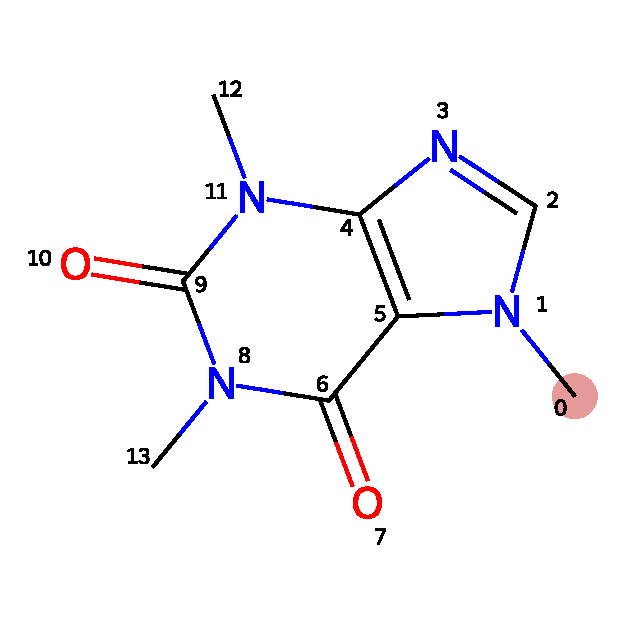
\includegraphics[width=\textwidth]{caffeine-atom0-fp0.pdf}
        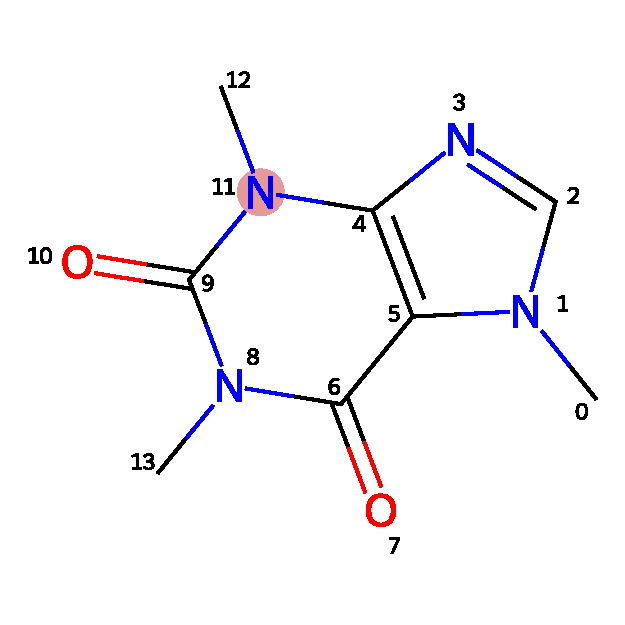
\includegraphics[width=\textwidth]{caffeine-atom11-fp0.pdf}
    \end{minipage}
    \begin{minipage}{0.22\textwidth}
        \centering
        $R=1$

        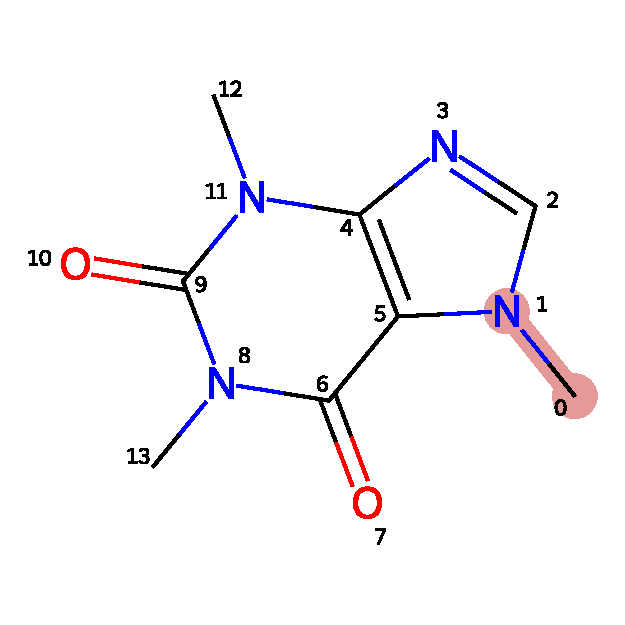
\includegraphics[width=\textwidth]{caffeine-atom0-fp1.pdf}
        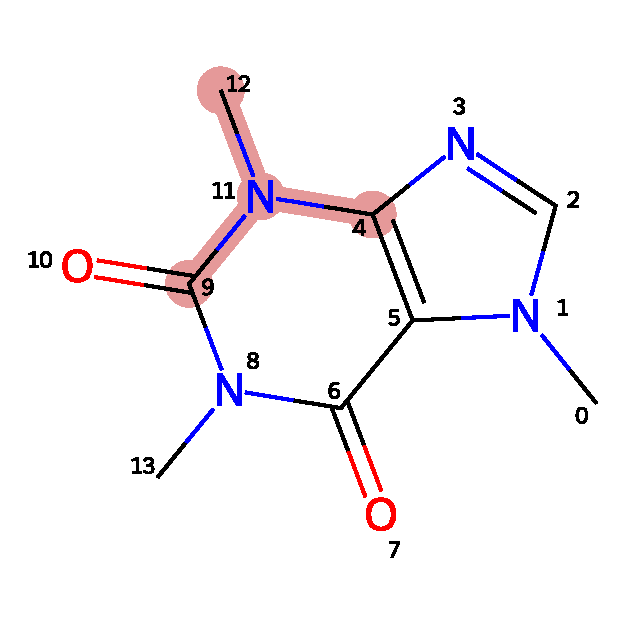
\includegraphics[width=\textwidth]{caffeine-atom11-fp1.pdf}
    \end{minipage}
    \begin{minipage}{0.22\textwidth}
        \centering
        $R=2$

        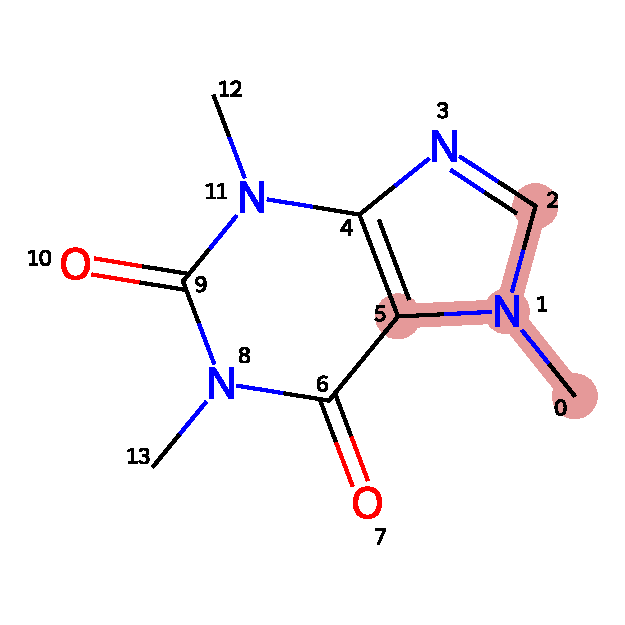
\includegraphics[width=\textwidth]{caffeine-atom0-fp2.pdf}
        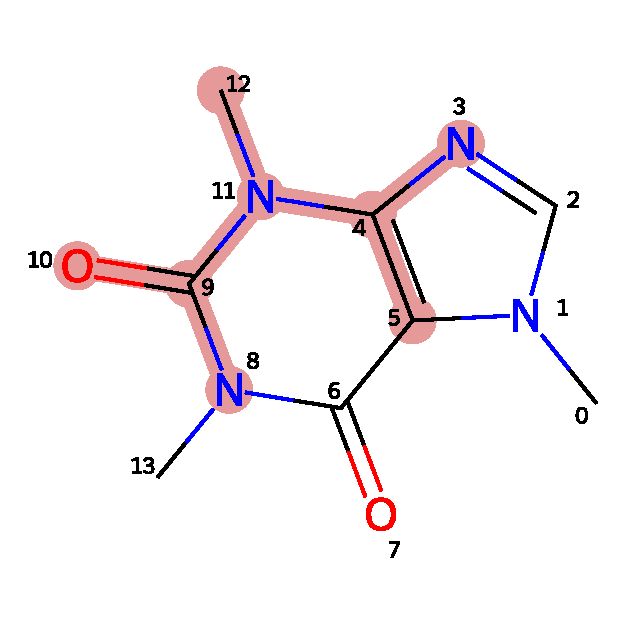
\includegraphics[width=\textwidth]{caffeine-atom11-fp2.pdf}
    \end{minipage}
    \begin{minipage}{0.22\textwidth}
        \centering
        $R=3$

        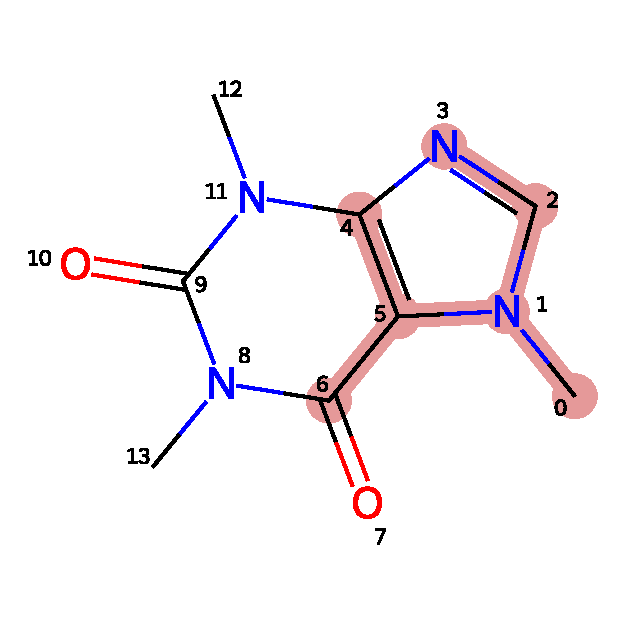
\includegraphics[width=\textwidth]{caffeine-atom0-fp3.pdf}
        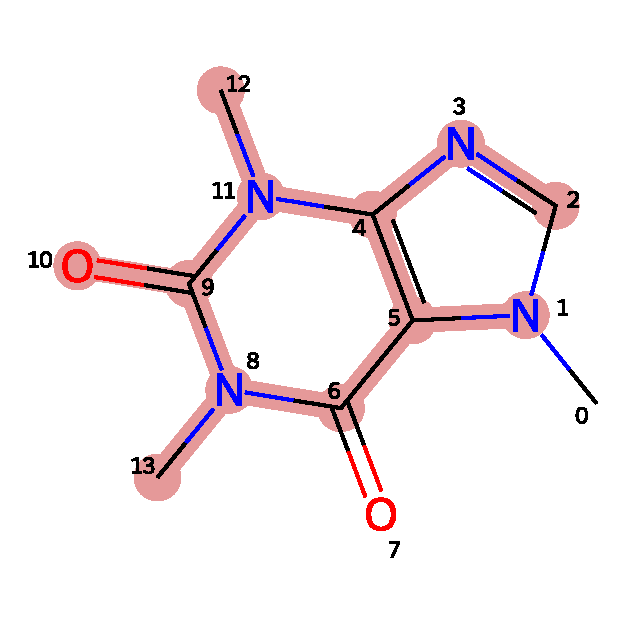
\includegraphics[width=\textwidth]{caffeine-atom11-fp3.pdf}
    \end{minipage}
    \caption[Illustration of subgraphs in Morgan fingerprints.]{
        Illustration of subgraphs of radius $0$ to $3$ around two atoms in caffeine
        (the carbon at index $0$ and the nitrogen at index $11$).
        Morgan fingerprints of radius $R=3$ would typically include the union of all such subgraphs
        for \emph{all atoms} (not just atoms $0$ and $11$) for \emph{all radii} from $0$ to $3$ (inclusive).
    }
    \label{fig:morgan-fp-example}
\end{figure}

\subsubsection{Post-processing multi-sets of subgraphs}

Post-processing consists of modifying the multi-set
and (optionally) converting the multi-set into a sparse vector.
The simplest kind of post-processing is the identity operator:
the multi-set is not modified, just returned as is.
Other common operations include discarding duplicate elements (thereby converting the multi-set into a plain set),
merging similar elements,\footnote{For example, paths with identical length and terminal atoms in atom-pair fingerprints.}
modifying elements,\footnote{For example, some implementations of Morgan fingerprints mask the identifies of the outermost ring of atoms to only consider the number of outgoing bonds.}
or deleting elements.\footnote{For example, some implementations of Morgan fingerprints effectively delete the $r=0$ subgraphs which consist of single atoms.}
After these modifications, the fingerprint can optionally be returned as a set-valued fingerprint.
Alternatively, to convert a fingerprint into a $k$-dimensional vector,
a hash function is first used to convert each subgraph in the multi-set to an integer in $\{1,\ldots,k\}$,
effectively forming a multi-set of integers $F$.
Then,
letting $\1_{\text{condition}}$ denote the indicator function (which is $1$ if the condition is true and $0$ otherwise),
a $k$-dimensional vector $v$ is formed such that
\begin{equation*}
    v_i=\1_{ i \in F }  
\end{equation*}
(referred to as a \emph{binary} fingerprint)
or
\begin{equation*}
    v_i=\sum_{j\in F} \1_{i = j}
\end{equation*}
(referred to as a \emph{count} fingerprint).
Note that count fingerprints differ from binary fingerprints only in the value of the non-zero indices
but not their location.
The vector $v$ is then returned as the fingerprint.

\subsubsection{Implementations of fingerprints}

In practice, implementations of fingerprinting algorithms may omit or combine certain steps for efficiency.
For example, most implementations of Morgan fingerprints directly compute hashes of subgraphs instead of forming
an explicit set of subgraphs.
Throughout this thesis fingerprint computations are handled by the third-party \texttt{rdkit} library
which computes Morgan fingerprint vectors of arbitrary length and radius (using an internal hash function).
Ultimately, only the following properties will be relied upon in subsequent chapters:
\begin{enumerate}
    \item Since the main difference between fingerprints is the set of subgraphs indexed, the ``type'' of most fingerprints is the same.
        Therefore, algorithms can be largely agnostic to the exact kind of fingerprint used.
    \item Fingerprints can be post-processed into vectors of different lengths and types, meaning that different versions of the same fingerprint can exist
        (e.g.\@ binary and count fingerprints).
        One can freely convert between these versions given the original set-valued fingerprint.
        This conversion is sometimes done implicitly.
    \item Fingerprints are not (necessarily) unique. For example, two molecules with the same atom count may have the same Morgan fingerprint of radius $0$.
        Therefore, in general, one cannot recover a molecule from its fingerprint.
\end{enumerate}
